\documentclass[11pt]{beamer}
% Packages
\usepackage{beamer-german}

% Title etc.
\title{Einführung}
\subtitle{Analyse politischer Unterstützung in der quantitativen Forschungspraxis}
\date{29. Oktober 2021}
\author{B. Philipp Kleer}
\institute{Institut für Politikwissenschaft | Justus-Liebig-Universität Gießen}

\setbeamerfont{itemize/enumerate body}{size = \small}
\setbeamerfont{itemize/enumerate subbody}{size = \footnotesize}
\setbeamerfont{itemize/enumerate subsubbody}{size = \scriptsize}

% Datumspaket
\usepackage[german]{isodate}

% Table packages
\usepackage{booktabs}
\usepackage{longtable}

\addbibresource{lit-s1.bib}

\begin{document}

\begin{frame}
	\maketitle
\end{frame}

\begin{frame}[t]{Heutige Agenda}
	\begin{itemize}
		\item Formalia (Termine, Stundenplan, Workload, Leistungsnachweise)
		\item Theoretische \& praktische Sitzungen
		\item Sitzungsvorbereitung
		\item Thematische Einführung
	\end{itemize}
\end{frame}

\begin{frame}[t]{Termin}
Wir treffen uns alle zwei Wochen an folgenden Uhrzeiten im \shine{selben} Webex-Raum:
	\begin{itemize}
		\item 10:00 Uhr bis 11:30 Uhr 
		\item 12:30 Uhr bis 14:00 Uhr
	\end{itemize}
\end{frame}

\begin{frame}[t]{Studienverlauf \& Vorwissen}
	\begin{center}
		\begin{figure}[ht]
			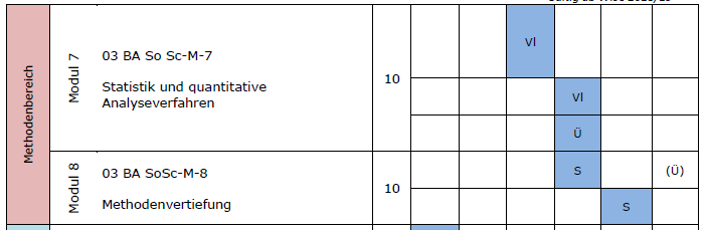
\includegraphics[width=\textwidth]{pics/pre1.png}
			\caption{\textbf{BA-Studium}}
		\end{figure}
	\end{center}
\end{frame}

\begin{frame}[t]{Seminarziel: BA}
	\begin{figure}[ht]
		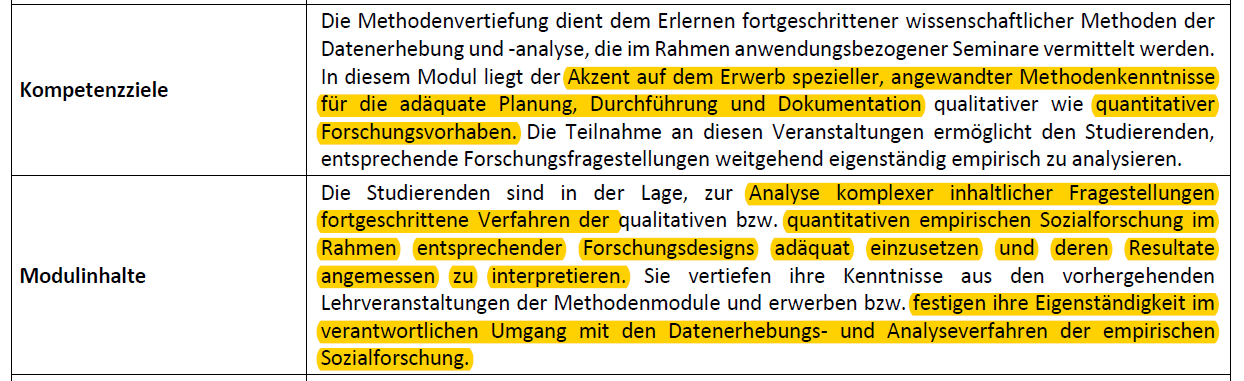
\includegraphics[width=\textwidth]{pics/pre2.png}
		\caption{\textbf{BA-Studium}}
	\end{figure}
\end{frame}

\begin{frame}[t]{Seminarziel}
Bei regelmäßiger und aktiver Teilnahme können Sie am Ende des Semesters: \\
	
	\begin{itemize}
		\item die Konzeption von politischer Unterstützung und politischer Kultur verstehen, erklären und in eigenen Analysen anwenden,\pause
		\item eine eigene kleine empirische Analyse planen (Theoriebezug, Forschungsfrage, Untersuchungsgegenstand, Methodenschritte)\pause
		\item eine selbstständig geplante empirische Analyse umsetzen (Studierende mit MAP)\pause
	\end{itemize}

\shine{Wie viel Sie tatsächlich von diesem Kurs mitnehmen, hängt davon ab, wie viel Sie reingeben!}
\end{frame}

\begin{frame}[t]{Workload}
	\begin{figure}[ht]
		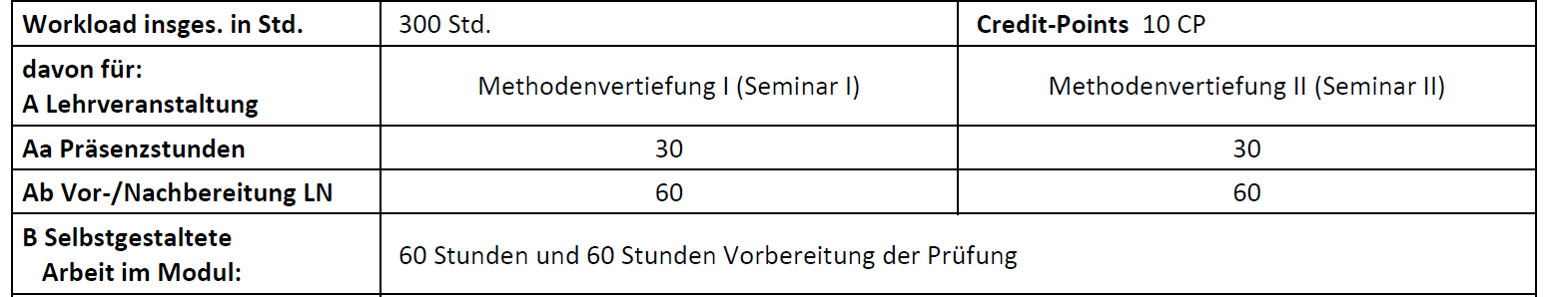
\includegraphics[width=\textwidth]{pics/pre4.png}
		\caption{\textbf{BA-Studium}}
	\end{figure}
\end{frame}

\begin{frame}[t]{As it is written, so it shall be done}
\underline{Anforderungen kleiner Schein} (BA-Studierende ohne MAP):
	\begin{itemize}
		\item Einführung in einen der theoretischen oder empirischen Texte (Zuteilung in 1. Sitzung)
		\item Mitarbeit in Planung eines Forschungsprojekts
		\item Peer-Feedback zu Forschungsideen anderer 
	\end{itemize}
\end{frame}

\begin{frame}[t]{As it is written, so it shall be done}
\underline{Anforderungen großer Schein} (BA-Studierende mit MAP):
	\begin{itemize}
		\item Vorstellung des geplanten Projekts in den letzten drei Einheiten (Theorie, Analyseschritte, evtl. erster Code)
		\item Abgabe einer Hausarbeit basierend auf der Projektidee (Formalia der Hausarbeit siehe Dokument in ILIAS)
	\end{itemize}
\end{frame}

\begin{frame}[t]{Wiederholungsprüfung}
Allgemeine Bestimmungen über modularisierte Studiengänge: \\
	\begin{itemize}
		\item § 19 Abs. 2, AllB: Studierende müssen \shine{Wiederholungstermine zum nächstmöglichen Termin} antreten und gelten insofern als angemeldet. Andernfalls gilt das Modul als endgültig nicht bestanden.
		\item § 22 Abs. 7, AllB: Thema der Hausarbeit darf gleich bleliben
		\item § 9 Abs. 3 SpezO: 2 Wiederholungsprüfungen möglich; 1. Wiederholungsprüfung entspricht in Form, Umfang und Dauer der nicht bestandenen Prüfungsleistung
		\item[$\Rightarrow$] Durchgefallen? 4-Wochen-Überarbeitungsfrist!
	\end{itemize}
\end{frame}

\begin{frame}[t]{Sprechstunde}
Die Sprechstunde ist vor allem für Studierende, die die MAP bzw. Prüfungsleistung in diesem Kurs erbringen, hilfreich, da hier individuelle Probleme breiter diskutiert werden können. Ebenso sollte bis Ende Februar eine Fragestellung für die Hausarbeit festgelegt werden. 

\end{frame}

\begin{frame}[t]{Sprechstunde}
	\begin{columns}
		\begin{column}{0.5\textwidth}
		\begin{figure}[ht]
		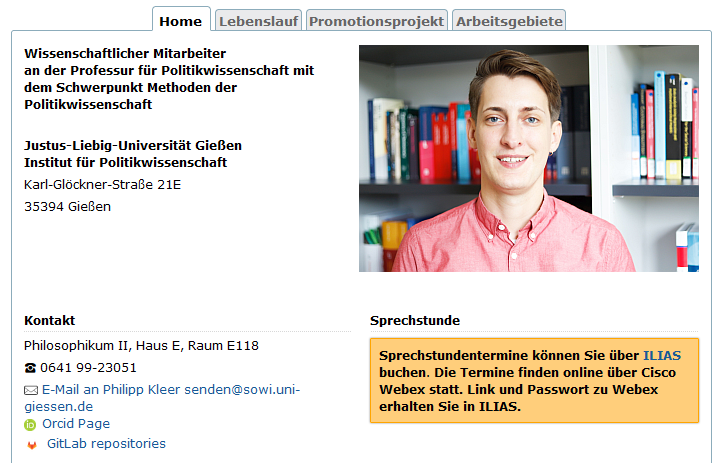
\includegraphics[width=\textwidth]{pics/pre6.png}
		\caption{\textbf{MA-Studium}}
	\end{figure}
		\end{column}
		\begin{column}{0.5\textwidth}
			Sie können über meine JLU-Homepage den \href{https://ilias.uni-giessen.de/ilias/goto.php?target=usr_172921&client_id=JLUG}{\textbf{Link zu ILIAS}} nutzen. Sie gelangen automatisch zu der Seite, auf der Sie sich für die Sprechstunde anmelden können.
		\end{column}
	\end{columns}
\end{frame}

\begin{frame}[t]{Hausarbeit}
	\begin{itemize}
		\item Formalia und Bewertungsmaßstab sind in ILIAS einsehbar (Objekteblock Allgemeine Informationen)
		\item Fragestellung, die in Hausarbeit untersucht werden soll, sollte bis zum 28.02.2022 in der Sprechstunde abgesprochen werden (nicht per E-Mail!)
		\item auch das Skript des jeweiligen Statistikprogramms muss abgegeben werden 
		\item sind die Daten nicht zugänglich, müssen auch diese mit abgegeben werden (Replikation ihrer Datenanalyse)
	\end{itemize}
\end{frame}

\begin{frame}[t]{Tonight you performed as group, and you will be judged as group!}
	\begin{itemize}
		\item Sie entscheiden sich \shine{bis 17. Dezember 2021}, ob Sie als Gruppe oder einzeln präsentieren wollen und bis Vorlesungsende (\shine{18. Februar 2022}), ob Sie die Hausarbeit als Gruppe oder einzeln schreiben möchten
		\pause
		\item für beides gilt: wenn keine Gruppenmeldung vorliegt $\Rightarrow$ Einzel-Präsentation/-Hausarbeit
		\pause
		\item (Gruppen-)Hausarbeit Umfang:
		\pause
			\begin{itemize}
				\item Einzeln: 4.000 Wörter (ca. 12 Seiten, max. 15)
				\item 2 Personen: 5.200 Wörter (ca. 16 Seiten, max. 20)
				\item 3 Personen: 6.600 Wörter (ca. 20 Seiten, max. 25)
				\item 4 Personen: 7.900 Wörter (ca. 24 Seiten, max. 30)
				\item mehr als vier Personen sind nicht erlaubt 
			\end{itemize}
		\pause
		\item eine Gruppe wird als Gruppe bewertet und nicht einzeln
	\end{itemize}
\end{frame}

\begin{frame}[t]{Abgabetermine}
Eine \textit{Deadline} ist eine \textit{Deadline} ist eine \textit{Deadline}. \\

Von Beginn der Veranstaltung sind die Abgabefristen kommuniziert, ich erwarte daher, dass diese eingehalten werden. Damit es für alle fair und gleich kommuniziert ist: Es gibt keine individuellen Verlängerungen.

\pause

Deadline für die Hausarbeiten ist der \shine{31.03.2022, 23:59 Uhr}. Es werden nur digitale Abgaben akzeptiert. Der Upload ist in ILIAS freigeschaltet. Die Hausarbeit muss als PDF hochgeladen werden, die Eigenständigkeitserklärung muss Teil dieses PDFs sein! Als zweite Datei muss das Skript aus dem Statistikprogramm hochgeladen werden. 

\end{frame}

\begin{frame}[t]{Sitzungen}
	\begin{center}
		\begin{figure}[ht]
			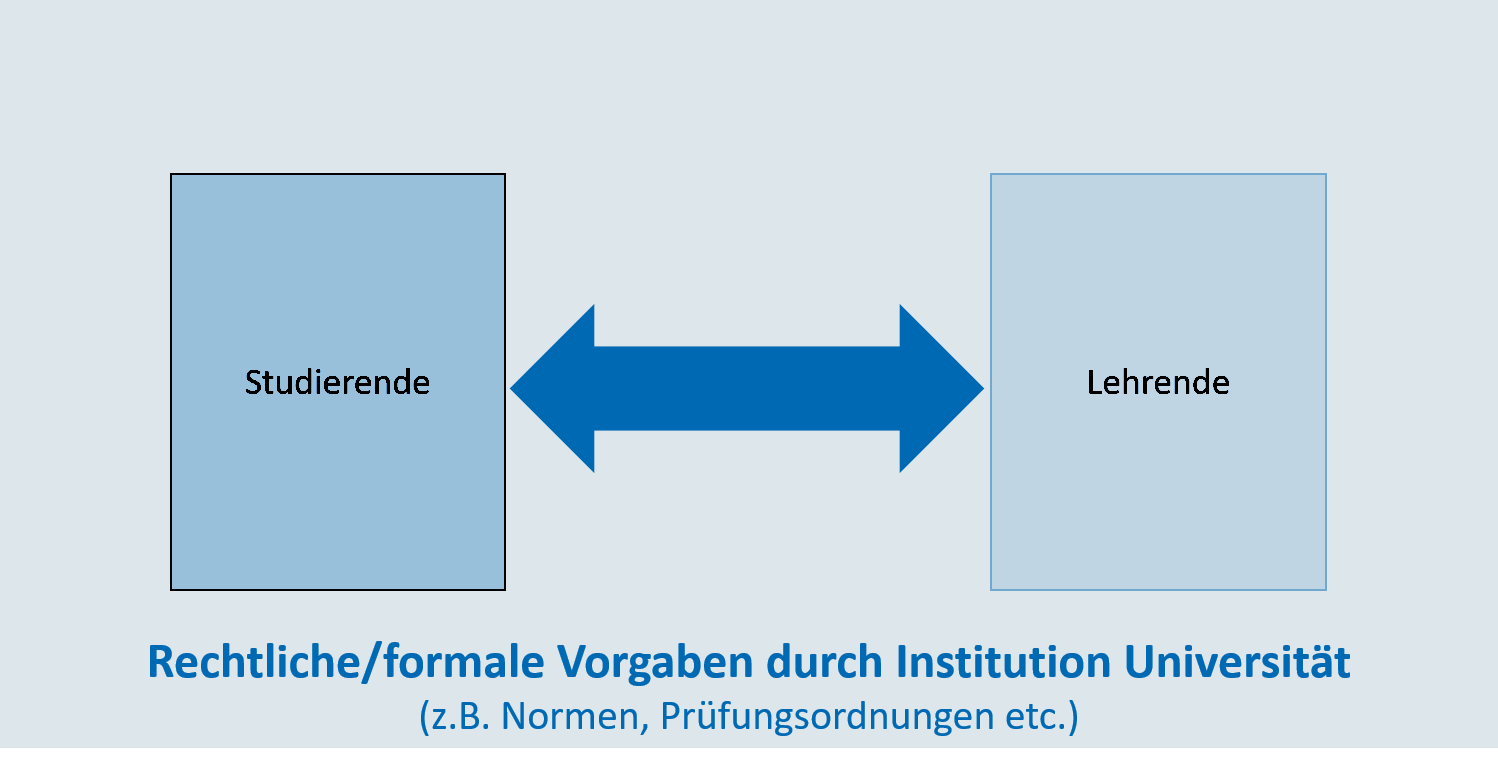
\includegraphics[width=\textwidth]{pics/pre7.png}
		\end{figure}	
	\end{center}
\end{frame}

\begin{frame}[t]{Sitzungen}
\shine{Was erwarte ich als Dozent?}

	\begin{itemize}
		\item Lesen/Vorbereiten der Texte, auch wenn man den Text nicht vorstellt
		\item kollegiales Miteinander
		\item respektvoller Umgang miteinander (vor allem bei der Vorstellung von Projektideen)
		\item Kursmaterialien alle über ILIAS erhältlich
		\item keine Sonderregelungen, für alle gelten gleiche Regelungen und Deadlines
		\item In der Ansprache ziehe ich das \shine{Du} vor
		\pause
		\item[$\Rightarrow$] meine Rolle: Unterstützer/Helfer, aber \underline{nicht} Motivator, Erzieher oder neuer bester Freund
	\end{itemize}
\end{frame}

\begin{frame}[t]{Warum seid ihr hier?}
Nun seid ihr an der Reihe: Wir machen eine kurze Vorstellungsrunde. 

Bitte nennt kurz euren Namen, in welchem Semester ihr seid und warum ihr diesen Kurs gew�hlt habt. 
\end{frame}

\begin{frame}[t]{Euer Erwartungsanspruch?}
Öffne den Browser und geh in die Lernumgebung in ILIAS. \\

Führe dort die Umfrage aus!
\end{frame}

\begin{frame}[t]{Rückfragen?}
	\begin{center}
		\begin{figure}[ht]
			
\includegraphics[width=\textwidth]{pics/pre8.png}
		\end{figure}	
	\end{center}
\end{frame}

\begin{frame}[t]{Semesterprogramm I}
\begin{nolist}
		\item[1.] Einheit: \printdate{2021-10-29}, Einführung ins Semesterprogramm, Einteilung der Texte (\textit{kleiner Schein})
		\item[2.] Einheit: \printdate{2021-10-29}, Politische Unterstützung \pause
		\item[3.] Einheit: \printdate{2021-11-12}, Politische Kultur
		\item[4.] Einheit: \printdate{2021-11-12}, Hands-On: Items finden und deskriptive Statistik \pause
		\item[5.] Einheit: \printdate{2021-11-26}, Politisches Vertrauen
		\item[6.] Einheit: \printdate{2021-11-26}, Hands-On: Korrelation \& Zusammenhangsmaße \pause
		\item[7.] Einheit: \printdate{2021-12-10}, Politisches Wissen \& Interesse
		\item[8.] Einheit: \printdate{2021-12-10}, Hands-On: Grafische Darstellungen \pause
\end{nolist}
\end{frame}

\begin{frame}[t]{Semesterprogramm II}
	\begin{nolist}
		\item[9.] Einheit: \printdate{2022-1-21}, Werte \& Wertewandel		
		\item[10.] Einheit: \printdate{2022-1-21}, Hands-On: Lineare Regression \pause
		\item[11.] Einheit: \printdate{2022-2-4}, Authoritarian Notions of Democracy
		\item[12.] Einheit: \printdate{2022-2-4}, Hands-On: Logistische Regression \pause
		\item[13.] Einheit: \printdate{2022-2-18}, Projektpräsentationen I
		\item[14.] Einheit: \printdate{2022-2-18}, Projektpräsentationen II 
	\end{nolist}
\end{frame}

\begin{frame}[t]{Texteinteilung}
	\begin{center}	
		\begin{table}
			\begin{tabular}{l l l}
			\toprule[2pt]
			Sitzung & Text & Textexperte(n)\\
			\midrule
			\multirow{2}{*}{29.10.2021} &\cite{Easton1975} & \\
			\cmidrule{2-3}
			& \cite{Fuhse2005} & \\
			\midrule
			\multirow{3}{*}{12.11.2021} & \cite[Kap. 1]{Almond1963} & \\
			\cmidrule{2-3}
			& \cite[Kap. 15]{Almond1963} & \\
			\cmidrule{2-3}
			& \cite{Gabriel2009} & \\
			\midrule
			\multirow{4}{*}{26.11.2021} & \cite{Festenstein2019} & \\
			\cmidrule{2-3}
			& \cite{Zmerli2020}  & \\
			\cmidrule{2-3}
			& \cite{Hooghe2017} & \\
			\bottomrule[2pt]
			\end{tabular}
		\end{table}
	\end{center}
\end{frame}

\begin{frame}[t]{Texteinteilung}
	\begin{center}	
		\begin{table}
			\begin{tabular}{l l l}
			\toprule[2pt]
			Sitzung & Text & Textexperte(n)\\
			\midrule
			\multirow{4}{*}{10.12.2021} & \cite{vanDeth2004} & \\
			\cmidrule{2-3}
			& \cite{Westle2020} & \\
			\cmidrule{2-3}
			& \cite{Reichert2019} & \\
			\cmidrule{2-3}
			& \cite{Russo2017} & \\
			\midrule
			\multirow{2}{*}{21.01.2022} & \cite[Kap. 1]{Welzel2013} & \\
			\cmidrule{2-3}
			& \cite{Inglehart2010} \\
			\midrule
			04.02.2022 & \cite[Kap. 10]{Welzel2013} & \\
			\bottomrule[2pt]
			
			\end{tabular}
		\end{table}
	\end{center}
\end{frame}

\begin{frame}{Teaser}
	\begin{columns}
		\begin{column}{0.5\textwidth}
			\begin{center}
				\begin{figure}[ht]
					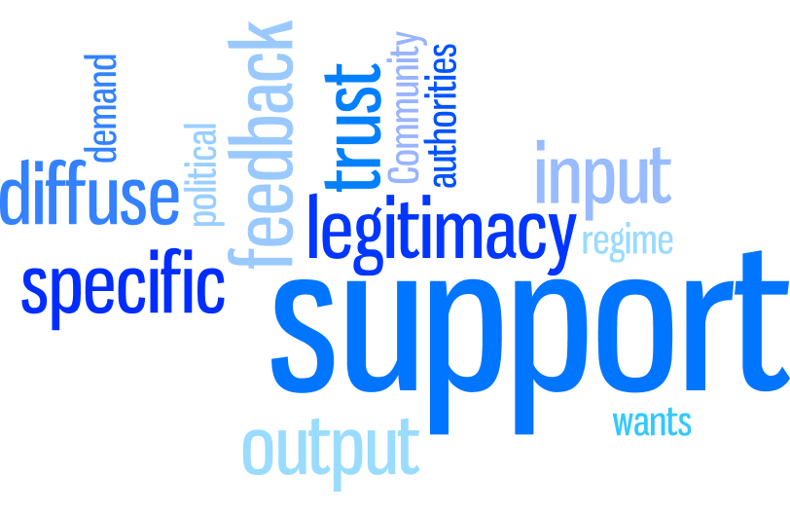
\includegraphics[width=\textwidth]{pics/pre9.png}
				\end{figure}	
			\end{center}
		\end{column}
		\begin{column}{0.5\textwidth}
			\begin{center}
				\begin{figure}[ht]
					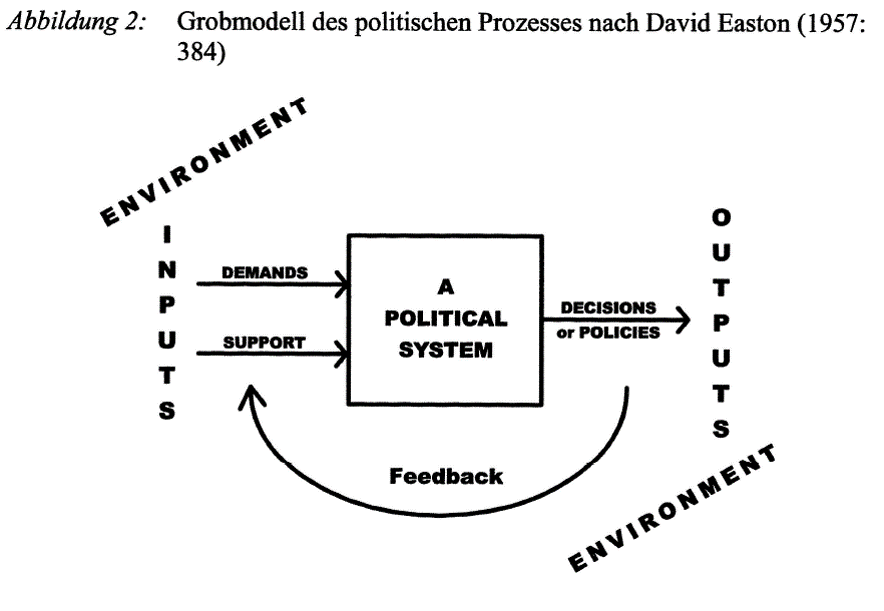
\includegraphics[width=\textwidth]{pics/pre10.png}
					\caption{Fuhse 2005: 35.}
				\end{figure}	
			\end{center}		
		\end{column}
				
	\end{columns}
\end{frame}

\begin{frame}[t]{SPSS-Zugang}
	\begin{itemize}
		\item Falls Sie einen Zugang zu SPSS benötigen, schreiben Sie mir bis \shine{Mittwochabend 18 Uhr} eine E-Mail (Name \& s-Kennung) von ihrer Uni-E-Mail-Adresse
		\item Für Sie wird der VPN-Zugang aktiviert und wenn Sie sich mit dem VPN-Zugang verbinden, können Sie SPSS von Zuhause aus nutzen (Installation des Programms vorausgesetzt)
	\end{itemize}
\end{frame}

\begin{frame}{Tipps zu SPSS}
	\begin{columns}
		\begin{column}{0.5\textwidth}
			\begin{center}
				\begin{figure}[ht]
					
\includegraphics[width=\textwidth]{pics/pre11.png} \pause
				\end{figure}	
			\end{center}
		\end{column}
		\begin{column}{0.5\textwidth}
			\begin{center}
				\begin{figure}[ht]
					
\includegraphics[width=\textwidth]{pics/pre12.png}
				\end{figure}	
			\end{center}		
		\end{column}
				
	\end{columns}
\end{frame}

\begin{frame}{Umstieg leicht gemacht!}
	\begin{center}
	Ein Web-Based-Training ist in ILIAS verlinkt.\\
				\begin{figure}[ht]
					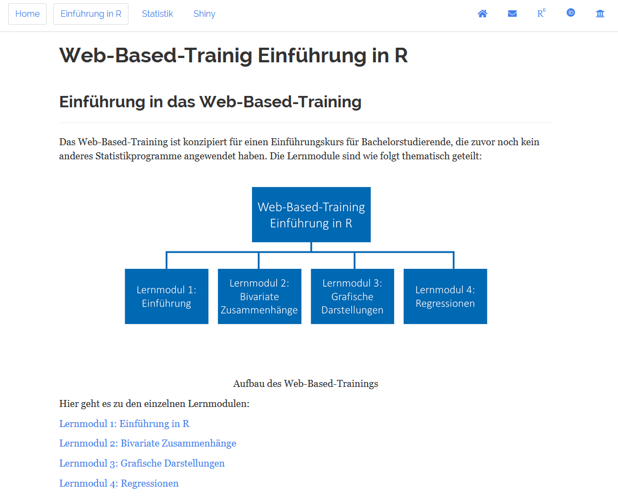
\includegraphics[width=0.8\textwidth]{pics/pre13.png}
				\end{figure}	
			\end{center}		
\end{frame}

\begin{frame}{Bei Rückfragen gilt immer: Semesterplan \& Texte}
	\begin{center}
				\begin{figure}[ht]
					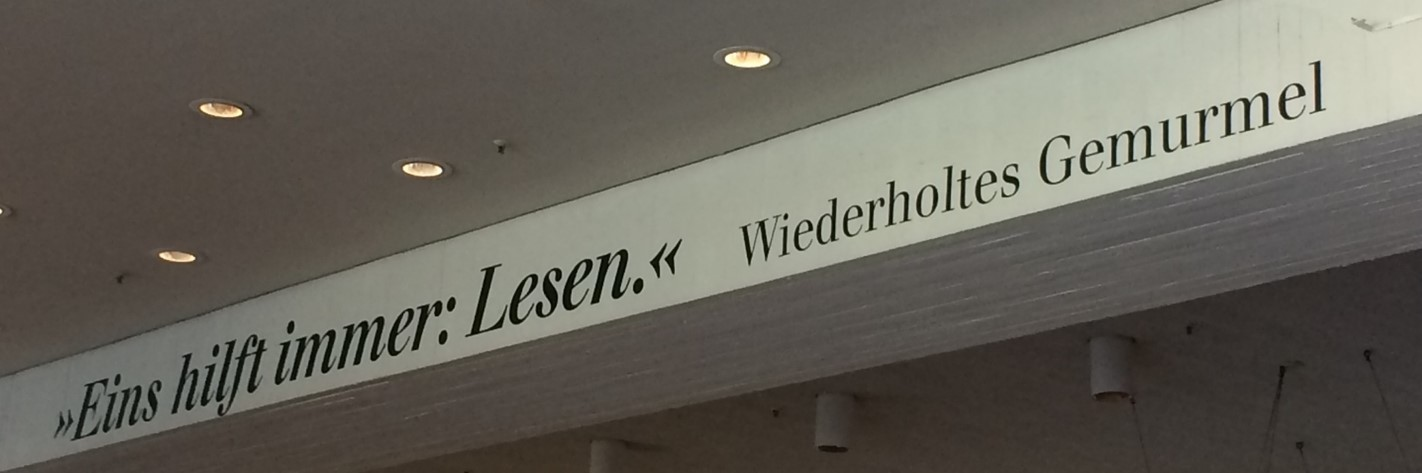
\includegraphics[width=\textwidth]{pics/pre14.png}
					\caption{Foyer der Staatsbibliothek zu Berlin (Haus Potsdamer Platz)}
				\end{figure}	
			\end{center}		
\end{frame}

\section{Mittagspause! \\ Wir treffen uns um 12:30 Uhr wieder.}

\begin{frame}[allowframebreaks]{Literatur}
	\nocite{*}
	\printbibliography[heading = none]
\end{frame}

\end{document}